Without any point of reference, the task of finding tight
and efficiently computable upper bounds
on the sensitivities seems rather challenging.
How are we supposed to find those ominous bounds and on top of that,
how can we make sure that their sum will be small?
It helps to remind ourselves of the original problem that the sensitivities
were designed to solve. Instead of sampling every point with equal
probability, the sensitvities were introduced to include the importance
of each point into the sampling process.
But what if similar importance distributions already existed?
Could it be possible to choose an existing importance distribution
and relate it to the concept of sensitivities in order to
obtain upper bounds?

It turns out, that there is one importance sampling
distribution that is particularly helpful in the context of our problem:
The so-called statistical leverage scores (see for example
\cite{leverage-scores-drineas}).
For a dataset $\mathcal{D} = \{(x_i, y_i)\}_{i=1}^n$ with model
matrix $X$, the statistical leverage score of the $i$-th observation is
given by $\ell_i = x_i^T(X^TX)^{-1}x_i$.
Intuitively speaking, $\ell_i$ is a measure of the uniqueness of a given
observation $x_i$. If there aren't many
data points close to $x_i$, i.e. we can consider $x_i$ to be
unique, then the leverage score of $x_i$
is high. On the other hand, if there are a lot of other data points
close to $x_i$, i.e. $x_i$ is not unique, then the leverage score
is low. When using leverage scores as a sampling distribution, we
give a higher weight to points that are unique and different from
the other points, compared to points that are surrounded by a lot
of similar other points.

To better understand what that means, a visualization of the statistical
leverage scores of an artificially generated two dimensional dataset
is given in figure~\ref{fig:leverage-scores} as an example.
We can see, that most of the datapoints that are crowding the
center of the dataset have rather low leverage scores, but the further
out the points are located relatively to the center, the higher
the leverage scores become.
Particularly, there is a small group of outliers in the
top right of the coordinate system, and we can see that their leverage
scores are almost four times as high as the leverage scores
of the points in the center. Thus, when sampling points proportionally
to their leverage scores, we are less likely to miss outliers in
the data that could potentially have a high impact on the loss function.

\begin{figure}[ht!]
    \centering
    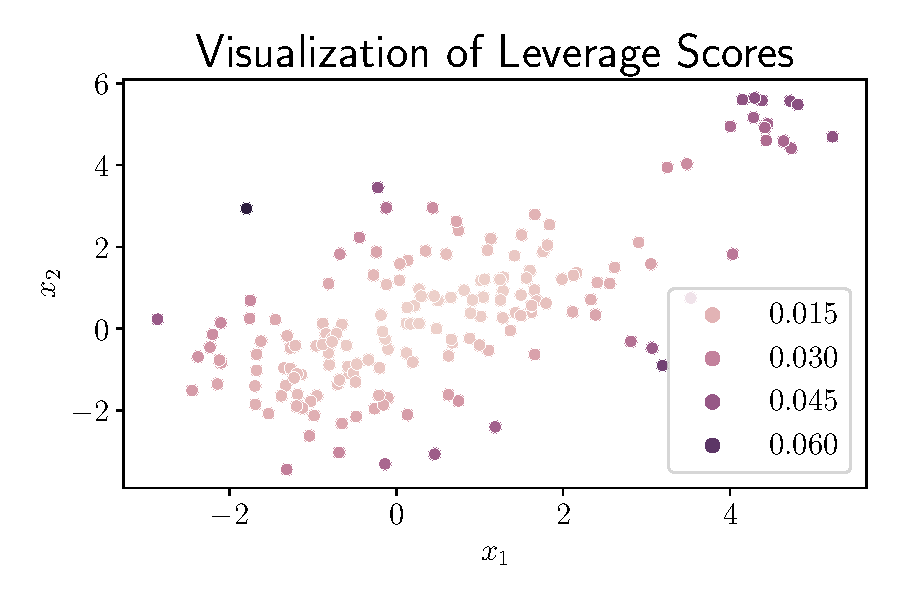
\includegraphics[width=.7\linewidth]{figures/leverage_scores_visualization.pdf}
    \caption{Visualization of the statistical leverage scores of an
        artificial two dimensional dataset. Darker colors indicate a higher
        leverage score than lighter colors.}
    \label{fig:leverage-scores}
\end{figure}

An alternative way of defining the leverage scores, which will
be particularly important to us when mathematically deriving
the sensitivity bounds later on, is to specify them as
the squared row norms of an orthonormal basis of the model matrix
$X \in \mathbb{R}^{n \times d}$.
Such an orthonormal basis can for example be obtained
by computing a so-called $QR$-decomposition of $X$
(see for example \cite{matrix-computations}), where
$X = QR$ is factorized into an orthonormal matrix
$Q \in \mathbb{R}^{n \times d}$ and an upper triangular
matrix $R \in \mathbb{R}^{d \times d}$.

Our goal in this section is to adapt the leverage scores in
such a way, that we can obtain tight upper bounds on the sensitivities.
But we are not quite ready for that yet.
Before we can get there, we first have to focus our attention back
to the probit loss function $g(x)$, because it turns out that in order
to bound the sensitivities by using the leverage scores, we first
have to cover some important properties of $g(x)$.

\subsubsection{A closer examination of the probit loss}

In order to find bounds on the sensitivities, we also
need bounds on the probit loss
$g(x) = \ln\left( \frac{1}{1 - \Phi(x)} \right)$.
The first bound that we will derive holds for all $x \geq 0$
and shows that $g(x)$ grows at least like a quadratic function.
Next, we will show that for all $x \geq 2$, $g(x)$ is upper
bounded by a quadratic function, and thus $g(x)$ asymptotically
grows like a quadratic function.
Both of these bounds will turn out to be helpful later
on. They are proven in lemma \ref{lemma:lower-bound}
and lemma \ref{lemma:upper-bound}.

\begin{lemma}
    \label{lemma:lower-bound}
    Let $g(x) = \ln \left( \frac{1}{1 - \Phi(x)}\right)$.
    Then, for all $x \geq 0$, it holds that:
    \begin{equation*}
        \frac{1}{2} x^2 \leq g(x).
    \end{equation*}
\end{lemma}
\begin{proof}
    We first show the claim for all $x \geq 1$, by using the following
    inequality:
    \begin{align*}
        \Phi(-x) & = \frac{1}{\sqrt{2 \pi}} \int_{-\infty}^{-x} \exp{ \left(-\frac{1}{2} t^2 \right)} dt       \\
                 & \leq \frac{1}{\sqrt{2 \pi}} \int_{-\infty}^{-x} -t \exp{ \left(-\frac{1}{2} t^2 \right)} dt \\
                 & = \frac{1}{\sqrt{2 \pi}} \exp{\left( -\frac{1}{2} x^2 \right)}                              \\
                 & \leq \exp{\left( -\frac{1}{2} x^2 \right)}.                                                 \\
    \end{align*}
    In the next step, we use this inequality to show that for $x \geq 1$:
    \begin{gather*}
        e^{g(x)} = e^{\ln \left( \frac{1}{1 - \Phi(x)} \right)} = \frac{1}{\Phi(-x)} \geq e^{\frac{1}{2} x^2}\\
        \iff \\
        g(x) \geq \frac{1}{2} x^2,
    \end{gather*}
    which proves the bound for $x \geq 1$.

    Let us now turn to the case when $0 \leq x \leq 1$.
    Both $g(x)$ and $\frac{1}{2}x^2$ are monotonically increasing
    and continuous functions for $0 \leq x \leq 1$.
    Making use of the fact that $g(0) > \frac{1}{2}$, it follows
    for all $0 \leq x \leq 1$, that
    \begin{equation*}
        g(x) \geq g(0) > \frac{1}{2} = \max_{0 \leq x \leq 1} \frac{1}{2} x^2 \geq \frac{1}{2} x^2,
    \end{equation*}
    which concludes the proof.
\end{proof}

\begin{lemma}
    \label{lemma:upper-bound}
    Let $g(x) = \ln \left(\frac{1}{1 - \Phi(x)}\right)$.
    Then, for all $x \geq 2$, it holds that:
    \begin{equation*}
        g(x) \leq x^2.
    \end{equation*}
\end{lemma}
\begin{proof}
    In~\cite{gaussian_bounds}, it was shown that the following inequality
    holds for all $x \geq 0$:
    \begin{equation*}
        \Phi(-x) \geq \frac{1}{\sqrt{2 \pi}} \frac{x}{x^2 + 1} e^{-\frac{1}{2} x^2}.
    \end{equation*}
    We can use this inequality to establish that for all
    $x \geq 2$ it holds that:
    \begin{align*}
        e^{x^2} \cdot \Phi(-x) & \geq e^{x^2} \frac{1}{\sqrt{2 \pi}} \frac{x}{x^2 + 1} e^{-\frac{1}{2} x^2}                           \\
                               & = e^{\frac{1}{2} x^2} \frac{1}{\sqrt{2 \pi}} \frac{x}{x^2 + 1}                                       \\
                               & = e^{\frac{1}{2} x^2} \frac{1}{\frac{4}{3}\left( x^2 + 1 \right)} \frac{\frac{4}{3} x}{\sqrt{2 \pi}} \\
                               & \geq \frac{e^{\frac{1}{2} x^2}}{\frac{4}{3}\left( x^2 + 1 \right)}                                   \\
                               & \geq \frac{e^{\frac{1}{2} x^2}}{e^{\frac{1}{2} x^2}}                                                 \\
                               & = 1                                                                                                  \\
        \iff                                                                                                                          \\
        e^{x^2}                & \geq \frac{1}{1 - \Phi(x)}                                                                           \\
        \iff                                                                                                                          \\
        x^2                    & \geq \ln \left(\frac{1}{1 - \Phi(x)}\right) = g(x),
    \end{align*}
    which completes the proof.
\end{proof}

\subsubsection{Finding the sensitivity bounds}

Having successfully established the quadratic bounds on the
probit loss $g(x)$, we can now turn our attention back to the
task of finding upper bounds on the sensitivities.
As already mentioned, we will be using the statistical leverage scores
in order to do so.

To this end, we will show that the function set $F = \{g_1, ..., g_n\}$,
which represents our dataset, can be partitioned into
two classes of functions for which we can find upper bounds
on the sensitivities.
The first class will contain all points, where the loss funcion
surpasses a specific threshold. It turns out, that
for a given $\beta$, the threshold $z_i^T \beta \geq 2$ is a suitable
candidate. In the next lemma, we show how we can relate the
loss function of all the points in this class to the
statistical leverage scores, while also incorporating $\mu$
into the upper bound. To do this, we use the notion of leverage
scores as the squared row norms of an orthogonal basis,
that can be obtained for example by conducting a $QR$-factorization.

\begin{lemma}
    \label{lemma:g-bounds-1}
    Let $\mathcal{D}$ be a $d$-dimensional and $\mu$-complex dataset of size
    $|\mathcal{D}|=n$ with scaled model matrix
    $Z \in \mathbb{R}^{n \times d}$ and let $w \in \mathbb{R}^n_{>0}$
    be a vector of positive weights.
    Let $F = \{g_1, ..., g_n\}$ be a set of functions with
    $g_i(\beta) = g(z_i^T \beta)$ and let
    $f_w(\beta) = \sum_{i=1}^n w_ig_i(\beta)$.
    Then, it holds that
    \begin{equation*}
        w_jg_j(\beta) \leq 2 \lVert U_j \rVert_2^2(1 + \mu)f_w(\beta) \quad
        \forall\ j \in \{i \in [n]:\ z_i^T \beta \geq 2 \},
    \end{equation*}
    where $U \in \mathbb{R}^{n \times d}$ is an orthonormal basis for
    the columnspace of $\sqrt{D_w}Z$ and $\sqrt{D_w} \in \mathbb{R}^{n \times n}$
    is a diagonal matrix, where the $i$-th diagonal element is equal to
    $\sqrt{w_i}$ and $U_j \in \mathbb{R}^d$ is the $j$-th row of $U$.
\end{lemma}
\begin{proof}
    Let $\sqrt{D_w} Z = UR$, where $U$ is an orthonormal basis for the columnspace
    of $\sqrt{D_w} Z$. Then, for all $j \in \{i \in [n]:\ z_i^T \beta \geq 2 \}$:
    \begin{equation*}
        w_jg_j(\beta) = w_j g(z_j^T \beta)
        = w_j g\left(\frac{\sqrt{w_j} z_j^T \beta}{\sqrt{w_j}}\right)
        = w_j g\left(\frac{U_j^T R \beta}{\sqrt{w_j}}\right)
        \leq w_j g\left(\frac{\lVert U_j \rVert_2 \lVert R \beta \rVert_2}{\sqrt{w_j}}\right),
    \end{equation*}
    where $U_j \in \mathbb{R}^d$ is the vector that constitutes the $j$'th
    row of $U$ and the inequality is true due to the
    \textit{Cauchy-Schwarz inequality}. We continue the proof as follows:
    \begin{align*}
        w_j g\left(\frac{\lVert U_j \rVert_2 \lVert R \beta \rVert_2}{\sqrt{w_j}}\right)
         & = w_j g\left(\frac{\lVert U_j \rVert_2 \lVert U R \beta \rVert_2}{\sqrt{w_j}}\right)          \\
         & = w_j g\left(\frac{\lVert U_j \rVert_2 \lVert \sqrt{D_w} Z \beta \rVert_2}{\sqrt{w_j}}\right) \\
         & \leq \lVert U_j \rVert_2^2 \lVert \sqrt{D_w} Z \beta \rVert_2^2                               \\
         & = \lVert U_j \rVert_2^2 \sum_{i=1}^n w_i (z_i^T \beta)^2.
    \end{align*}
    Here, the first equality follows from the fact that $U$ is orthonormal, i.e.
    multiplying by $U$ doesn't change the norm of a vector.
    The inequality follows from the bound $g(x) \leq x^2$ that holds for
    all $x \geq 2$, which was shown in lemma~\ref{lemma:upper-bound}.

    Now, let $I_\beta^+ = \{i \in [n]:\ w_i z_i^T \beta > 0 \}$
    and let $I_\beta^- = \{i \in [n]:\ w_i z_i^T \beta < 0 \}$ like in
    definition~\ref{def:mu}, the definition of $\mu$-complexity.
    We continue the proof by making use of the relationship that
    was shown in lemma~\ref{lemma:mu-inequalities}:
    \begin{align*}
        \lVert U_j \rVert_2^2 \sum_{i=1}^n w_i (z_i^T \beta)^2
         & = \lVert U_j \rVert_2^2 \left( \sum_{i \in I_\beta^+} w_i (z_i^T \beta)^2 + \sum_{i \in I_\beta^-} w_i (z_i^T \beta)^2 \right)        \\
         & \leq \lVert U_j \rVert_2^2 \left( \sum_{i \in I_\beta^+} w_i (z_i^T \beta)^2 + \mu \sum_{i \in I_\beta^+} w_i (z_i^T \beta)^2 \right) \\
         & = \lVert U_j \rVert_2^2 (1 + \mu) \sum_{i \in I_\beta^+} w_i (z_i^T \beta)^2                                                          \\
         & \leq 2 \lVert U_j \rVert_2^2 (1 + \mu) \sum_{i \in I_\beta^+} w_i g(z_i^T \beta),
    \end{align*}
    where the last inequality follows from the bound
    $g(x) \geq \frac{1}{2}x^2$, that holds for all $x \geq 0$,
    which we proved in lemma~\ref{lemma:lower-bound}.

    From here, we can use the fact that $g$ is a strictly positive function
    to complete the proof:
    \begin{equation*}
        2 \lVert U_j \rVert_2^2 (1 + \mu) \sum_{i \in I_\beta^+} w_i g(z_i^T \beta)
        \leq 2 \lVert U_j \rVert_2^2 (1 + \mu) \sum_{i = 1}^n w_i g(z_i^T \beta)
        = 2 \lVert U_j \rVert_2^2 (1 + \mu) f_w(\beta)
    \end{equation*}
\end{proof}

In the next lemma, we turn to the remaining class of points where
$z_i^T \beta \leq 2$, and show how the sensitivity of these points
can be bounded by a constant value that only depends on $\mu$
and the weight of the given point.

\begin{lemma}
    \label{lemma:g-bounds-2}
    Let $\mathcal{D}$ be a $d$-dimensional and $\mu$-complex dataset of size
    $|\mathcal{D}|=n$ with scaled model matrix
    $Z \in \mathbb{R}^{n \times d}$ and let $w \in \mathbb{R}^n_{>0}$
    be a vector of positive weights.
    Let $F = \{g_1, ..., g_n\}$ be a set of functions with
    $g_i(\beta) = g(z_i^T \beta)$ and let
    $f_w(\beta) = \sum_{i=1}^n w_ig_i(\beta)$.
    Then, it holds that
    \begin{equation*}
        w_jg_j(\beta) \leq \frac{w_j}{\mathcal{W}}(80 + 16 \mu)f_w(\beta) \quad
        \forall\ j \in \{i \in [n]:\ z_i^T \beta \leq 2 \},
    \end{equation*}
    where $\mathcal{W} = \sum_{i=1}^n w_i$ is the sum of all weights.
\end{lemma}
\begin{proof}
    We first start by noting that $g(-1) > \frac{1}{10}$
    and that $g(2) < 4$. Now, we partition the indices into
    two sets as follows:
    \begin{gather*}
        K_\beta^- = \{ i \in [n] \ | \ z_i^T \beta \leq -1 \} \\
        K_\beta^+ = \{ i \in [n] \ | \ z_i^T \beta > -1 \}.
    \end{gather*}
    In the case that
    $\sum_{j \in K_\beta^+} w_j \geq \frac{1}{2} \mathcal{W}$, the following
    relationship holds:
    \begin{equation*}
        f_w(\beta) = \sum_{i=1}^n w_i g(z_i^T \beta)
        \geq \sum_{i \in K_\beta^+} w_i g(z_i^T \beta)
        \geq \frac{\sum_{i \in K_\beta^+} w_i}{10}
        \geq \frac{\mathcal{W}}{20}
        = \frac{\mathcal{W}}{20 w_j} w_j
        \geq \frac{\mathcal{W}}{80 w_j} w_j g(z_j^T \beta),
    \end{equation*}
    where $j \in \{i \in [n]:\ z_i^T \beta \leq 2 \}$.
    Thus, we have in this case:
    \begin{equation*}
        w_jg(z_j^T\beta) \leq \frac{80w_j}{\mathcal{W}} f_w(\beta).
    \end{equation*}

    \noindent If on the other hand
    $\sum_{j \in K_\beta^-} w_j \geq \frac{1}{2} \mathcal{W}$,
    we have that
    \begin{equation*}
        f_w(\beta)
        = \sum_{i=1}^n w_i g(z_i^T \beta)
        \geq \sum_{i \in I_\beta^+} w_i g(z_i^T \beta)
        \geq \frac{1}{2} \sum_{i \in I_\beta^+} w_i (z_i^T \beta)^2
        \geq \frac{1}{2\mu} \sum_{i \in I_\beta^-} w_i (z_i^T \beta)^2,
    \end{equation*}
    where $I_\beta^+ = \{i \in [n]:\ w_i z_i^T \beta > 0 \}$
    and $I_\beta^- = \{i \in [n]:\ w_i z_i^T \beta < 0 \}$ like in
    definition~\ref{def:mu} ($\mu$-complexity).
    The second inequality is true due to the lower bound
    $g(x) \geq \frac{1}{2} x^2$ that holds for all $x \geq 0$
    (see lemma~\ref{lemma:lower-bound}) and
    the third inequality is true due to a property of $\mu$ that
    was proved in lemma~\ref{lemma:mu-inequalities}.

    We continue the proof as follows:
    \begin{equation*}
        \frac{1}{2\mu} \sum_{i \in I_\beta^-} w_i (z_i^T \beta)^2
        \geq \frac{1}{2 \mu} \sum_{i \in K_\beta^-} w_i (z_i^T \beta)^2
        \geq \frac{1}{2 \mu} \sum_{i \in K_\beta^-} w_i
        \geq \frac{\mathcal{W}}{4 \mu}
        \geq \frac{\mathcal{W}}{16 \mu w_j} w_j g(z_j^T \beta),
    \end{equation*}
    which leads us to the upper bound for the second case:
    \begin{equation*}
        w_jg(z_j^T\beta) \leq \frac{16 \mu w_j}{\mathcal{W}} f_w(\beta).
    \end{equation*}

    We can conclude the proof by adding both upper bounds:
    \begin{equation*}
        w_j g_j(\beta)
        = w_j g(z_j^T \beta) \leq \frac{80 w_j}{\mathcal{W}} f_w(\beta)
        + \frac{16 \mu w_j}{\mathcal{W}} f_w(\beta)
        = \frac{w_j}{\mathcal{W}} (80 + 16 \mu) f_w(\beta).
    \end{equation*}
\end{proof}

It is now time to use the results from lemma~\ref{lemma:g-bounds-1}
and lemma~\ref{lemma:g-bounds-2} to derive an upper bound on
the sensitivities. Because we showed how the dataset can
be partitioned in "high loss points" and "low loss points"
for every given $\beta$ and how these two classes of points
can both be upper bounded, it simply suffices to add those
bounds together to bound the sensitivities for any given $\beta$.
As a final step, we only have to show that the total sum of the
sensitivities remains small. We do both in the following lemma.

\begin{lemma}
    \label{lemma:sensitivity-bounds}
    Let $\mathcal{D}$ be a $d$-dimensional and $\mu$-complex dataset of size
    $|\mathcal{D}|=n$ with scaled model matrix
    $Z \in \mathbb{R}^{n \times d}$, let $w \in \mathbb{R}^n_{>0}$
    be a vector of positive weights and let
    $U \in \mathbb{R}^{n \times d }$ be an orthonormal basis for
    the columnspace of $\sqrt{D_w}Z$.
    Let $F = \{g_1, ..., g_n\}$ be a set of functions with
    $g_i(\beta) = g(z_i^T \beta)$ and let
    $f_w(\beta) = \sum_{i=1}^n w_ig_i(\beta)$.
    Then, the sensitivity $\varsigma_i$ of $g_i$
    (see definition~\ref{def:sensitivity}) is upper bounded by
    \begin{equation*}
        \varsigma_i \leq s_i
        = (80 + 16\mu)(\lVert U_i \rVert_2^2 + \frac{w_i}{\mathcal{W}}),
    \end{equation*}
    and the total sensitivity is bounded by
    \begin{equation*}
        \mathfrak{S} = \sum_{i=1}^n \varsigma_i \leq 192 \mu d.
    \end{equation*}
\end{lemma}
\begin{proof}
    We can use the bounds that we derived in lemma~\ref{lemma:g-bounds-1}
    and lemma~\ref{lemma:g-bounds-2} to bound the sensitivities:
    \begin{align*}
        \varsigma_i
         & = \sup_{\beta \in \mathbb{R}^d,\ f_w(\beta)>0} \frac{w_i g(z_i \beta)}{f_w(\beta)}                   \\
         & \leq \sup_{\beta \in \mathbb{R}^d,\ f_w(\beta)>0} \frac{2 \lVert U_i \rVert_2^2 (1 + \mu) f_w(\beta)
            + \frac{w_i}{\mathcal{W}} (80 + 16 \mu) f_w(\beta)}{f_w(\beta)}                                     \\
         & = 2 \lVert U_i \rVert_2^2 (1 + \mu) + \frac{w_i}{\mathcal{W}} (80 + 16 \mu)                          \\
         & \leq \lVert U_i \rVert_2^2 (80 + 16 \mu) +  \frac{w_i}{\mathcal{W}} (80 + 16 \mu)                    \\
         & = (80 + 16\mu)(\lVert U_i \rVert_2^2 + \frac{w_i}{\mathcal{W}}),
    \end{align*}
    which completes the first part of the proof.
    For the next part, we use that $U$ is an orthonormal matrix.
    The Frobenius norm $\lVert U \rVert_F$
    (see for example~\cite{matrix-computations}) of an orthonormal matrix
    is equal to $\sqrt{d}$, as can easily be verified:
    \begin{equation*}
        \lVert U \rVert_F = \sqrt{\sum_{k=1}^d \sum_{l=1}^n \lvert u_{lk} \rvert^2}
        = \sqrt{\sum_{k=1}^d 1} = \sqrt{d},
    \end{equation*}
    where the second equality follows from the fact that the columns of
    $U$ have unit norm due to its orthonormality. We can now conclude the
    proof as follows:
    \begin{align*}
        \mathfrak{S}
         & = \sum_{i=1}^n \varsigma_i \leq (80 + 16\mu) \sum_{i=1}^n \lVert U_i \rVert_2^2 + \frac{w_i}{\mathcal{W}} \\
         & = (80 + 16 \mu)(\lVert U \rVert_F^2 + 1)                                                                  \\
         & = (80 + 16 \mu)(d + 1)                                                                                    \\
         & \leq 96 \mu(d + 1)                                                                                        \\
         & \leq 192 \mu d.
    \end{align*}
\end{proof}

We now have successfully completed the first task on our list of
developing a coreset construction algorithm by using the
sensitivity framework. Not only did we manage to derive upper bounds
on the sensitivities of the function set $F = \{g_1, ..., g_n\}$
that represents our dataset by using the
statistical leverage scores, but we also showed that
the sum of those bounds is in $O(\mu d)$, even independent of
the total number of datapoints $n$.
The final step, before putting everything together, is now to find
an upper bound of the VC-dimension of the range-space
induced by $F^\ast$.
